\documentclass[compress]{beamer}
\usetheme{metropolis}
\useinnertheme{rounded}
\useoutertheme{miniframes}
\usepackage[italian]{babel}
\definecolor{royalblue3}{RGB}{58,95,205}
\definecolor{giallo}{RGB}{197, 151, 0}
\definecolor{blu}{RGB}{19 101 158}
\setbeamercolor{section in head/foot}{fg=white, bg=blu}
\setbeamercolor{subsection in head/foot}{fg=blu, bg=blu!20}
\setbeamercolor{subsection in head/foot}{fg=blu, bg=blu!20}
\setbeamercolor{frametitle}{fg=blu, bg = white}
\setbeamercolor{title}{bg = white, fg=blu}
\setbeamercolor{author in head/foot}{bg=blu, fg=white}
\setbeamercolor{title in head/foot}{bg=blu!40, fg=blu}
\setbeamercolor{date in head/foot}{bg=blu!20, fg=blu}
\setbeamercolor{item}{fg=giallo}
\setbeamercolor{caption name}{fg=blu}
\usepackage{tikz}
\usetikzlibrary{positioning}
\usepackage{multirow}
\usepackage{tabularx}
\usepackage{setspace}
\usepackage{booktabs}
\usepackage{tikz}
\usepackage{mathtools}
\usepackage{atbegshi}

\title[\textsc{Statistica Psicometrica}]{\textsc{Guess the correlation}}
\author[]{Dr. Ottavia M. Epifania}
\date[]{\texttt{ottavia.epifania@unitn.it}}

\begin{document}
\begin{frame}[plain]
    \maketitle
\end{frame}

\begin{frame}
	
	
	\begin{overprint}
		\centering
		\onslide<1> 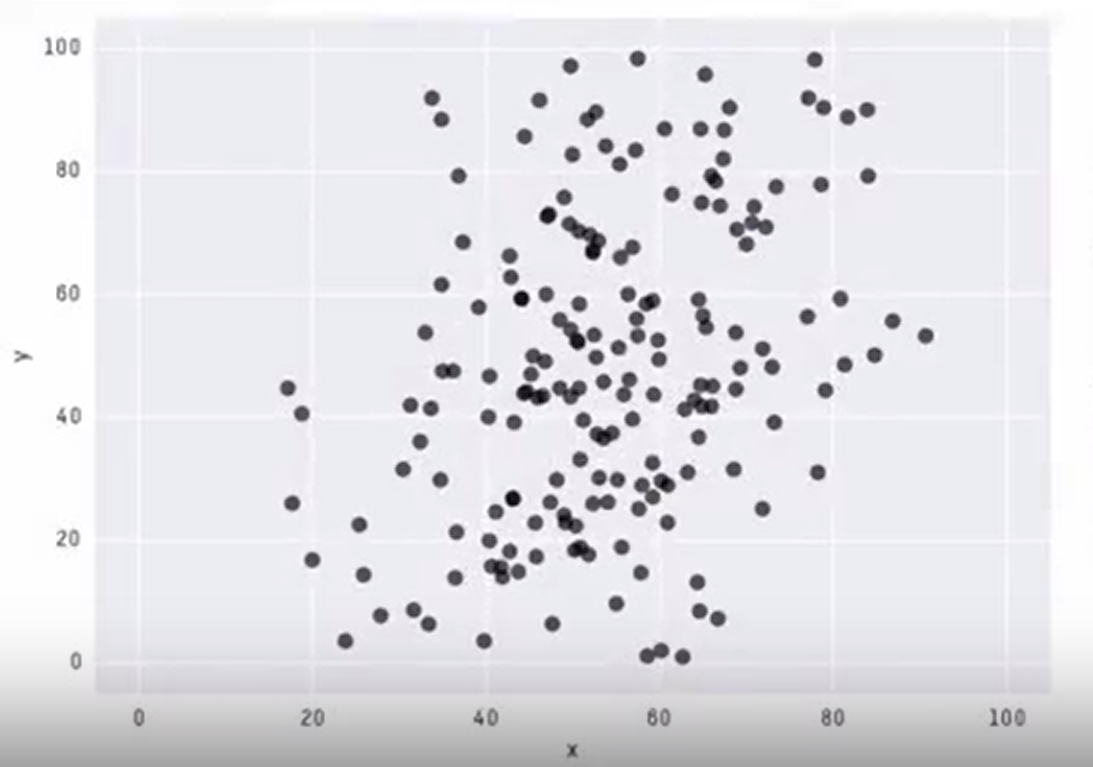
\includegraphics[width=\linewidth]{general_corr}
\onslide<2>	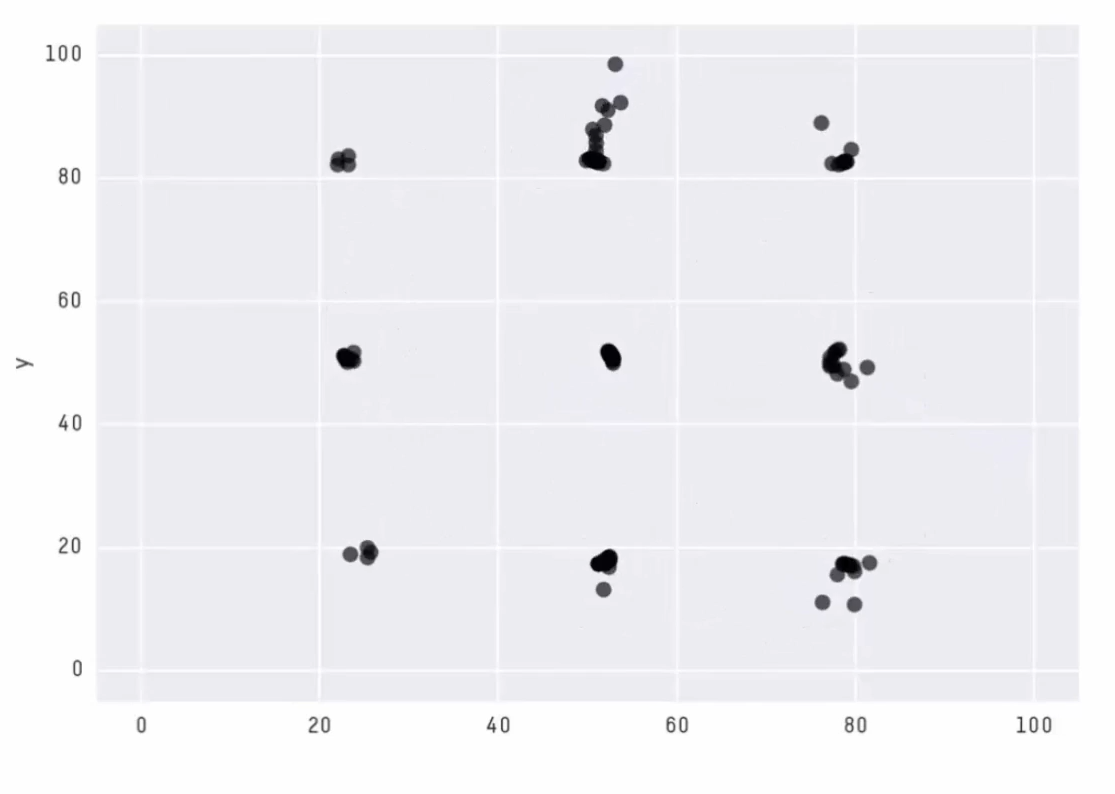
\includegraphics[width=\linewidth]{points}
\onslide<3>	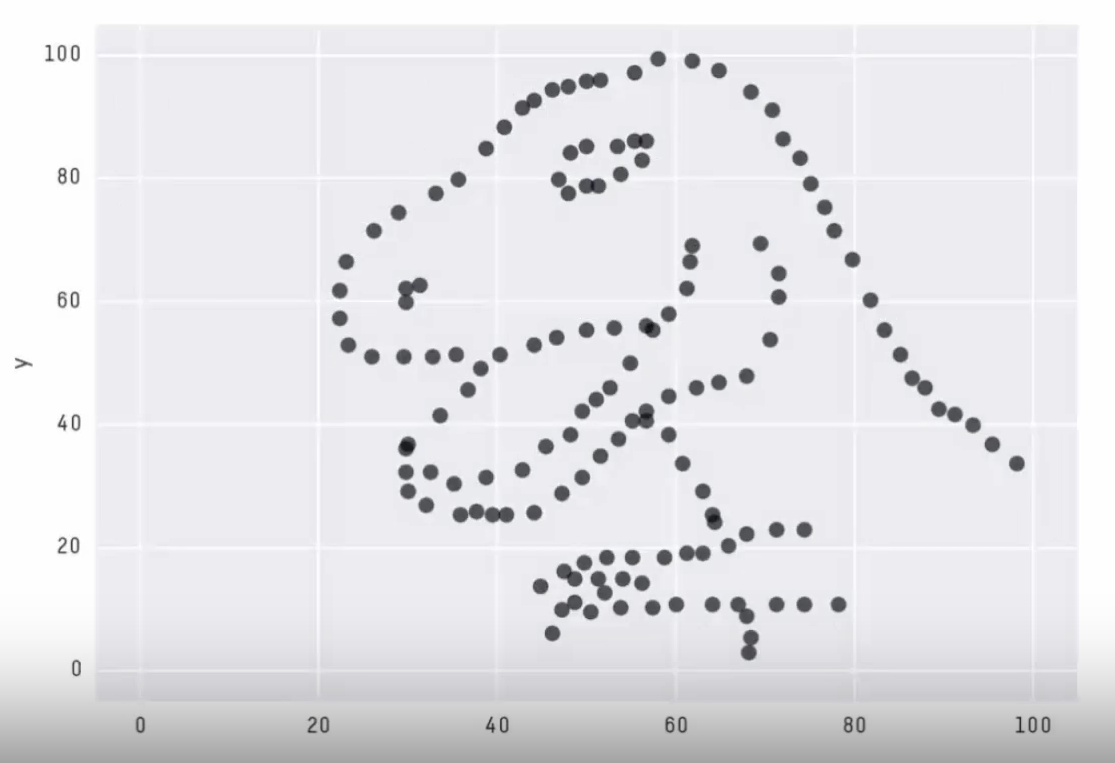
\includegraphics[width=\linewidth]{trex}
\onslide<4>	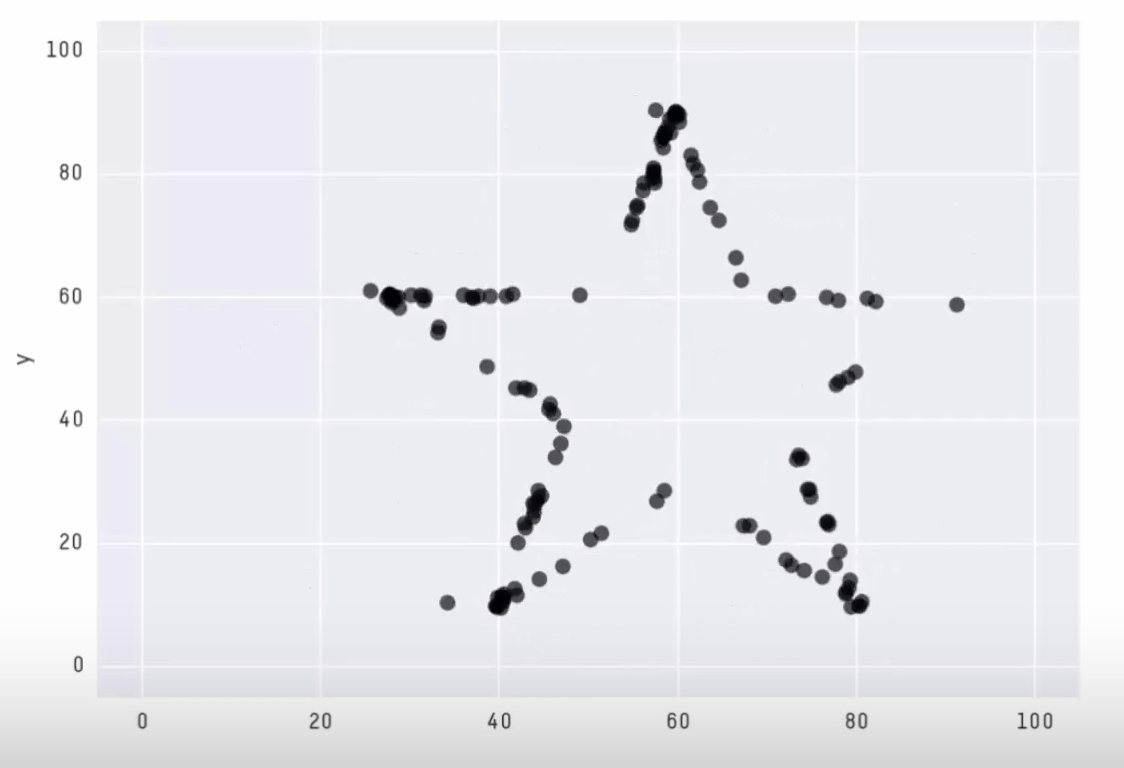
\includegraphics[width=\linewidth]{star}
	\onslide<5>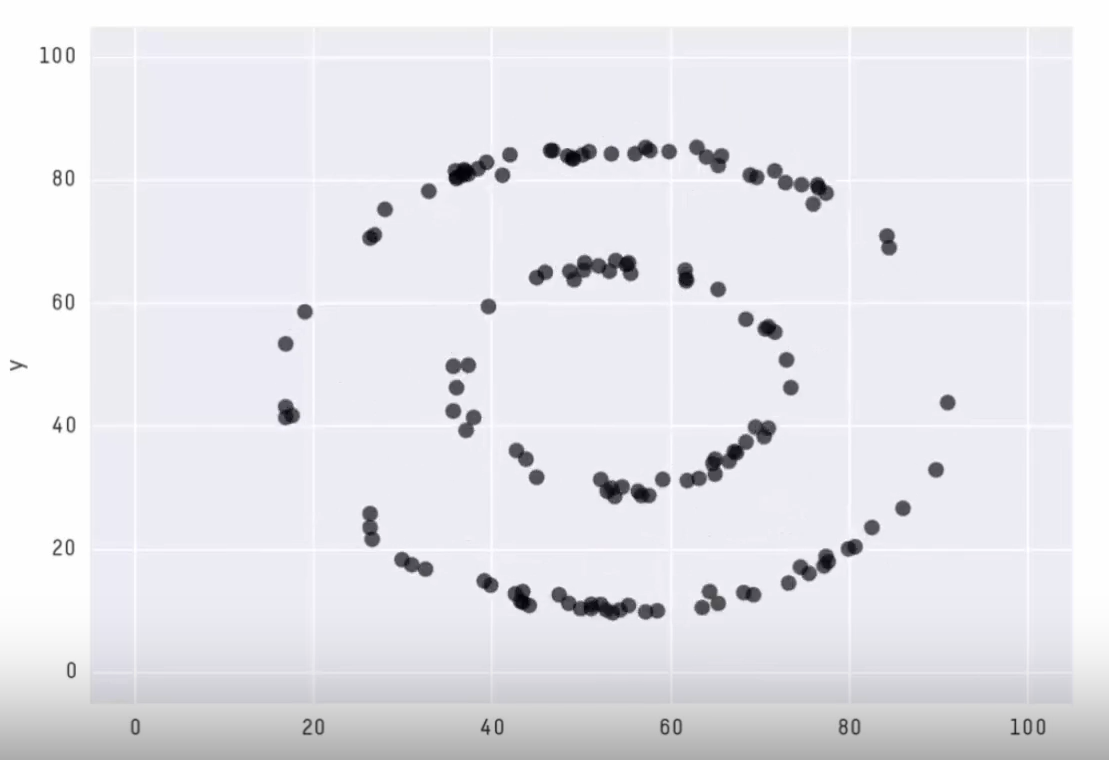
\includegraphics[width=\linewidth]{eye}


		
	\end{overprint}
\end{frame}

\begin{frame}
	\begin{columns}[T]
		\begin{column}{.50 \linewidth}
				\centering	
						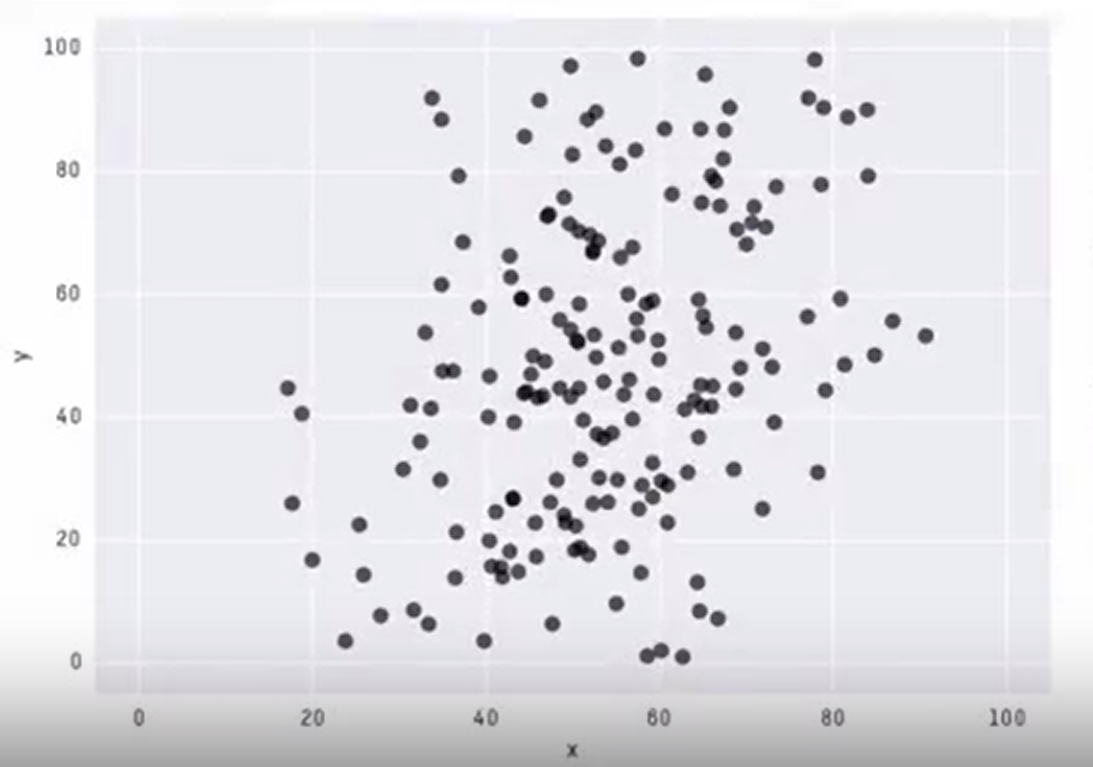
\includegraphics[width=.6\linewidth]{general_corr}
				
				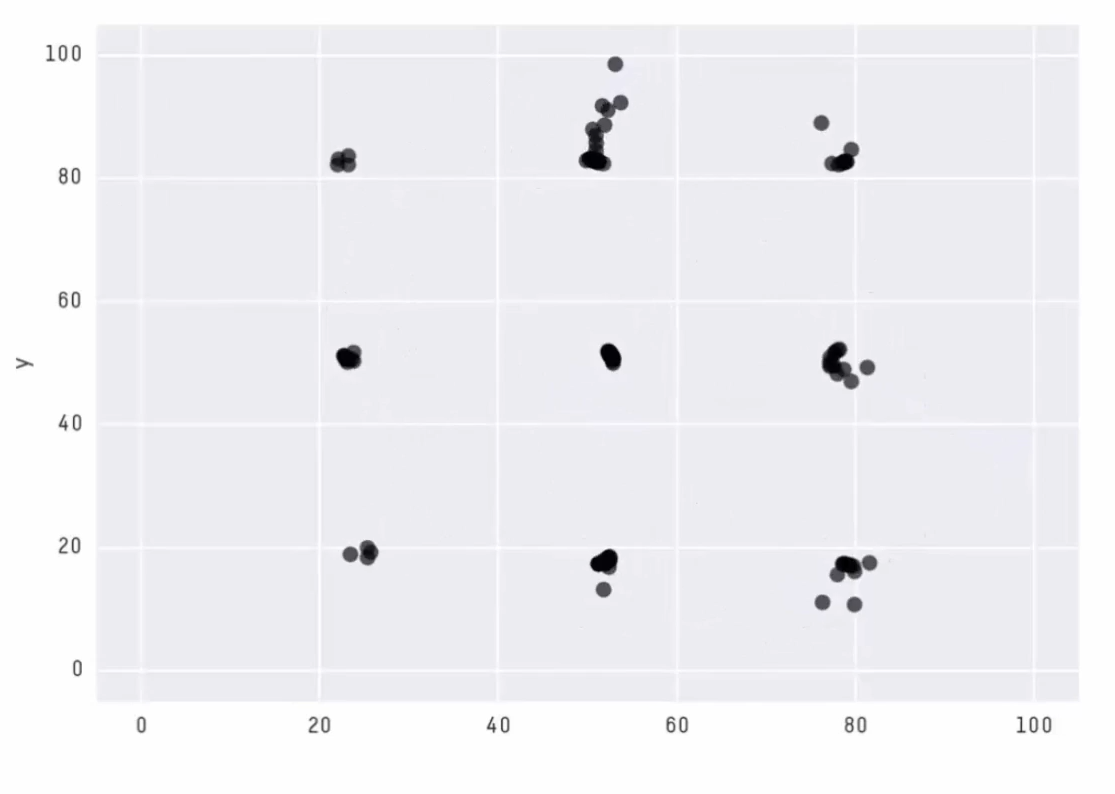
\includegraphics[width=.6\linewidth]{points}

				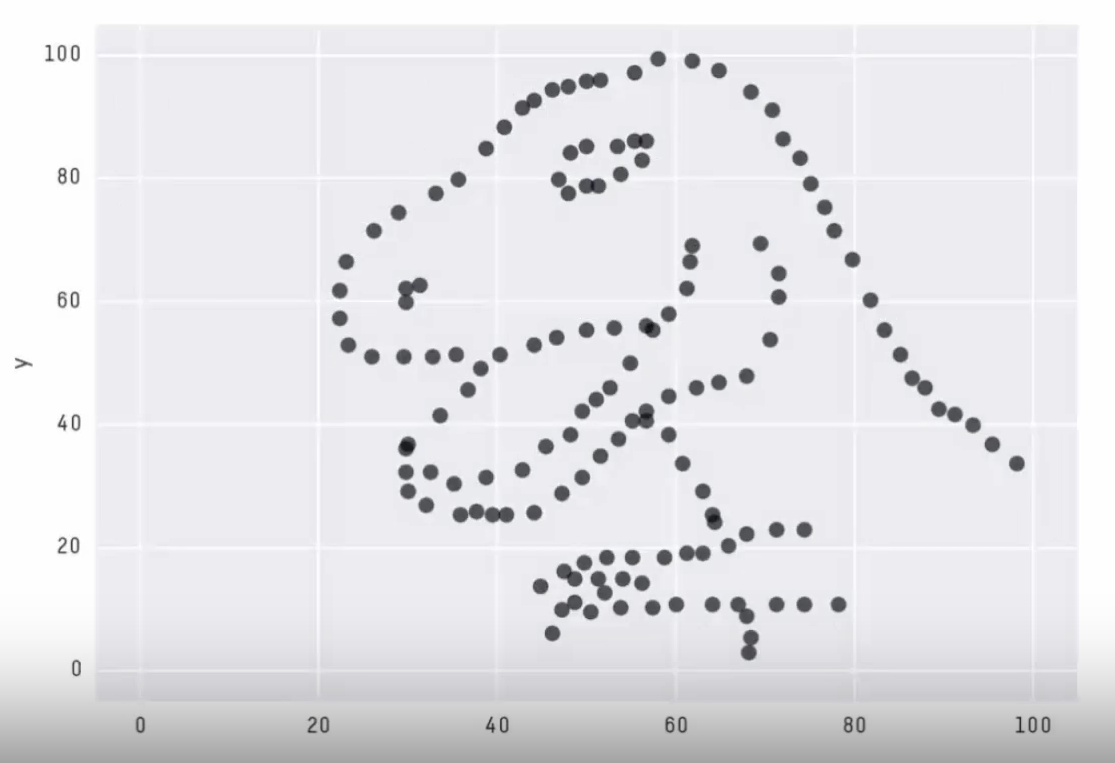
\includegraphics[width=.6\linewidth]{trex}
		\end{column}
		
			\begin{column}{.50 \linewidth}
				\centering	
				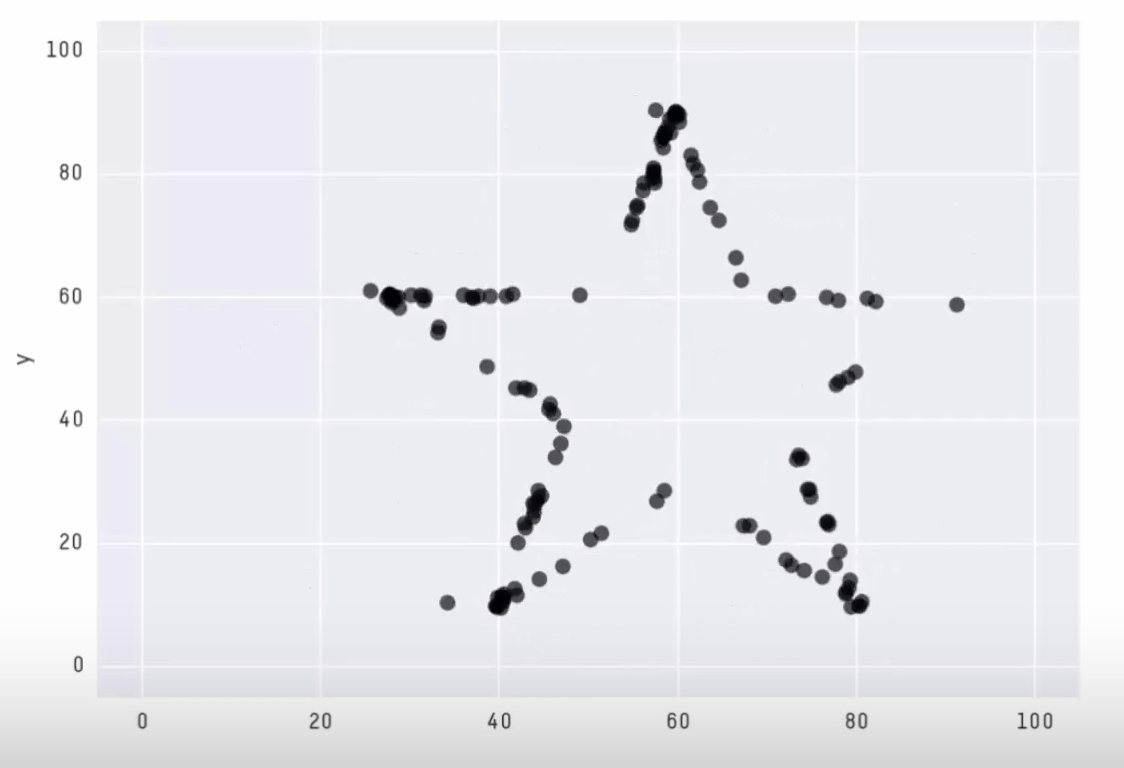
\includegraphics[width=.6\linewidth]{star}

				\centering	
				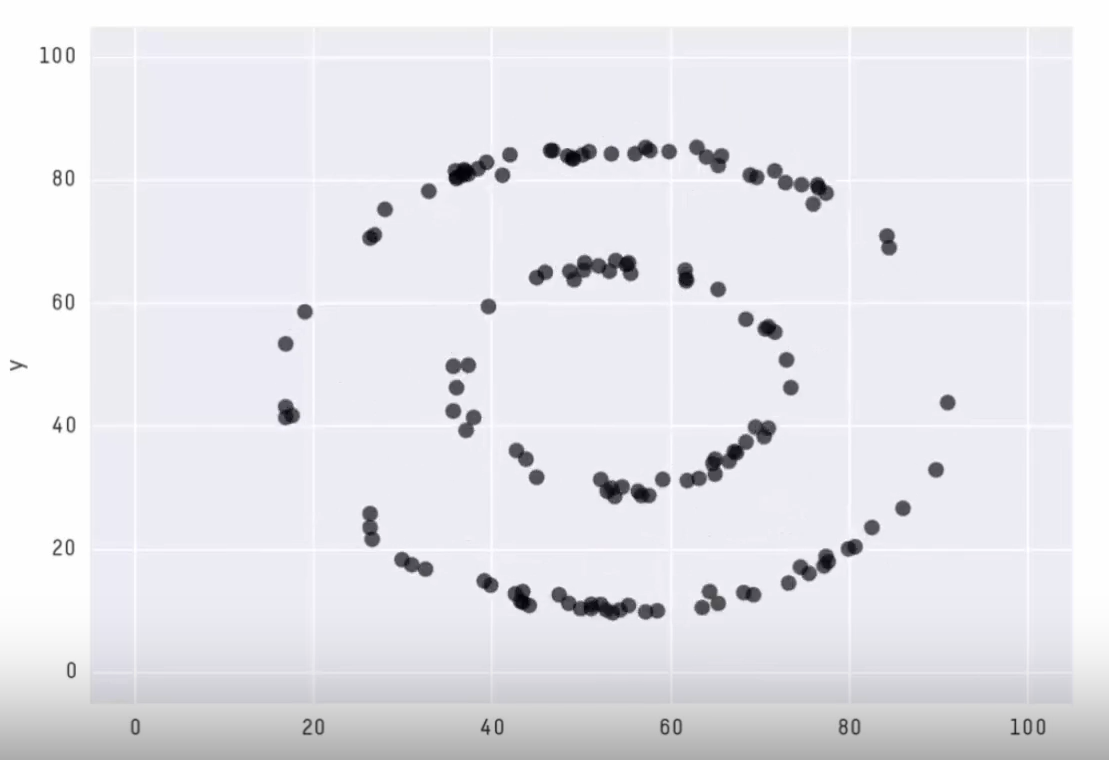
\includegraphics[width=.6\linewidth]{eye}
				
				\pause
				\begin{table}
					\centering
					\begin{tabular}{p{1.5cm} p{3.5cm}}
						$\bar{X}$ & $54.26 \pm 16.76$ \\
						$\bar{Y}$ & $47.83 \pm 26.93$ \\
						$r_{xy}$ & $-0.06$\\
					\end{tabular}
				\end{table}
		\end{column}
	\end{columns}
	
	
	
	
	
	\url{https://doi.org/10.1145/3025453.3025912}
\end{frame}

\end{document}
